\chapter{CONCEPTOS PRELIMINARES}

% ---------------> conjuntos, funciones y sucesiones
\section{Conjuntos, funciones y sucesiones}

En adición a los conjuntos de puntos que se trabajan con normalidad
en Matemáticas ~---puras y aplicadas---, se tendrá que hacer uso
frecuentemente de los conjuntos de conjuntos, si por ejemplo $X$ es
la recta real, como un intervalo es un conjunto de puntos, es decir
un subconjuto de $X$, se tendrá que el conjunto de todos los
intervalos es un conjunto de conjuntos.

En especial, cuando una clase hace referencia a subconjuntos del
conjunto $X$, la llamaremos \textbf{familia}. En especial el
\textbf{conjunto potencia} $\mathcal{P} (X)=\{A\mid A\subseteq X\}$
es una familia de $X$. Asimismo, se definirá el \textbf{complemento}
de $A$ por \[A^c=\{x\mid x\notin A\}.\]

\begin{defn}\label{dfcp28} Una \textbf{función de selección}
para un conjunto $X$ es una función $f$ la cual asocia a cada
subconjunto no vacío $E$ de $X$ un elemento de $E$: $f(E)\in E$.
\end{defn}

\begin{axm}[de selección]\label{choice} Para cualquier conjunto
existe una función de selección.
\end{axm}

\begin{rem} Con frecuencia el axioma~\ref{choice} se presenta en
la forma: para cada $E\in \mathcal{P}(X)\setminus\{\nada\}$,
elegimos un elemento $x\in E$. Asimismo, es equivalente al lema de
Zorn, para más detalles consultar
~\cite[p. 97]{Halmo},~\cite[p. 338]{Haus} o~\cite[p. 14]{Hewit}.
\end{rem}

Una \textbf{clase disjunta} es una clase {\boldmath $A$} de
conjuntos tal que para cualquier par de conjuntos distintos de
{\boldmath $A$} son disjuntos, en este caso nos referiremos a la
unión de conjuntos de {\boldmath $A$} como \textbf{unión disjunta}.

Si $E$ es un subconjunto de $X$, la función $\chi _E$ definida para
$x\in X$ por la relación:
\begin{equation}\label{eq0}
    \chi_E(x)= \begin{cases}
    1, & \mbox{si } x\in E, \\
    0, & \mbox{si } x\notin E.
    \end{cases}
\end{equation}Es llamada \textbf{función característica}
del conjunto $E$. La correspondencia entre los conjuntos y sus
funciones características es inyectiva, y todas las propiedades de
conjuntos y operaciones entre conjuntos pueden ser expresadas por
medio de funciones características. 

%%%	TABLA CORTA, ÚNICAMENTE LLEVA LÍNEAS HORIZONTALES PARA SEPARAR BLOQUES

\begin{table}[ht]
\caption[título optativo de la tabla]{Propiedades de los espacios $L^p$. Fuente: tomada de \cite[Cap. 3]{Brez}.}\label{tablaLp}
\centering
\begin{tabular}{cccc}
\hline
Espacio & Reflexivo\footnote{En el sentido topológico.} & Separable & Dual \\ \hline %\hline
$L^p$, $1<p<\infty$  & Si & Si & $L^q$, $1/p+1/q=1$ \\
$L^1$ & No & Si & $L^\infty$ \\
$L^\infty$ & No & No & $L^1 \varsubsetneq (L^\infty)’$ \\ \hline
\end{tabular}
\end{table}\footnotetext{En el sentido topológico.} 

\begin{defn}\label{dfcp1}Si $\su En$ es una sucesión de
conjuntos, definiremos los conjuntos $\overline{\lim } E_n$ y
$\underline{\lim } E_n$ de la siguiente forma:
\[\begin{array}{cc}
  \overline{\lim} E_n=\limsup \limits_{n\rightarrow \infty}E_n =
  \bigcap \limits_{n=1}^\infty \Union Ein \infty ,&
  \underline{\lim} E_n=\liminf \limits_{n\rightarrow \infty}E_n =
  \bigcup \limits_{n=1}^\infty \Inter Ein \infty \\
\end{array}\] y los llamaremos \textbf{límite superior} y
\textbf{límite inferior}, respectivamente, de la sucesión $\su En$.
Si tenemos $\overline{\lim} E_n = \underline{\lim} E_n$, usaremos la
notación $\lim_n E_n$ para este conjunto. Si la sucesión es tal que
$E_n\subset E_{n+1},\ n=1,2,\dots$ le llamaremos \textbf{creciente}
y se denotará por $E_n\!\!\uparrow$ y su límite será $\lim
\limits_{n\rightarrow \infty}E_n = \union En1 \infty$; si es tal que
$E_n\supset E_{n+1},\ n=1,2,\dots$ le llamaremos
\textbf{decreciente} y se denotará por $E_n\!\!\downarrow$ y su
límite será $\lim \limits_ {n\rightarrow \infty}E_n = \inter En1
\infty$. En ambos casos nos referiremos a ella como
\textbf{monótona}.\end{defn}


\begin{defn}\label{dfcp2}Sea $f$ una aplicación definida del conjunto
$X$ al conjunto $Y$, es decir $f:X\To Y$. Para cualquier subconjunto
$T\subseteq Y$, definimos la \textbf{imagen inversa} de $T$, bajo
$f$, denotada por $\ff (T)$, como sigue:
\[\ff (T)=\{s\in X\mid f(s)\in T\}.\]\end{defn} 

\begin{thm}\label{thcp1}Para la aplicación $\ff :{\cal{P}} (Y)
\To {\cal{P}} (X)$ se tienen las propiedades siguientes:
\begin{enumerate}
    \vspace{-6pt} \item $\ff(\bigcup_j T_j) = \bigcup_j
    \ff(T_j)$.
    \vspace{-6pt} \item $\ff(\bigcap_j T_j) = \bigcap_j
    \ff(T_j)$.
    \vspace{-6pt} \item Si $T_1\cap T_2=\nada$, entonces
    $\ff(T_1)\cap \ff(T_2) = \nada$.
    \vspace{-6pt} \item $\ff(T^c) = [\ff(T)]^c$.
    \vspace{-6pt} \item $\ff(\nada) = \nada$.
    \vspace{-6pt} \item $\ff(Y) = X$.
\end{enumerate}
\end{thm}


Las propiedades (1) y (3) del teorema~\ref{thcp1} establecen las
condiciones para la unión disjunta en una familia en $Y$. Sea ahora
$\Df$ una familia cualquiera de subconjuntos de $Y$, y definamos la
familia $\ff (\Df)$ de subconjuntos de $X$ como
sigue:\begin{equation}\label{eq1}
    \ff(\Df) = \{A\subseteq X \mid
A = \ff(T) \mbox{ para algún } T\in \Df\} = \{\ff(T) \mid T\in
\Df\}.
\end{equation}

El sistema de numeros reales extendido o \textbf{recta real
extendida} es el conjunto definido por $\RR\df\R \cup \{-\infty,
+\infty\}$, con la siguiente relación de orden: para $a\in \R$
tenemos $-\infty <a< +\infty$. La topología para este conjunto se
define por declarar como abiertos a los siguientes conjuntos:
$(a,b),\ [-\infty,b),\ (a,+\infty]$ y cualquier unión de conjuntos
de este tipo. Cuando se haga referencia a los \textbf{numeros reales
extendidos} o \textbf{valor real extendido}, se estará hablando de
los numeros reales y de los símbolos $\pm\infty$. Cuando trabajamos
con teoría de la integración, nos encontraremos con $\infty$, una
razón es que algunas veces trataremos de integrar sobre conjuntos de
medida infinita, este es caso de la recta real.

Por tal motivo, se hacen las siguientes definiciones para
facilitar su manejo: $a+\infty = \infty+a \df \infty$ si $0\leq a
\leq \infty$,~y
\begin{equation}\label{eq4}
    a\cdot \infty = \infty \cdot a
\df\begin{cases}
  \infty, & \mbox{si } 0 < a \leq \infty \\
  0, & \mbox{si } a = 0 \\
\end{cases}
\end{equation}las leyes de cancelación se tratan
así: $a+b = a+c\ \Rightarrow\ b=c\ $ y $a\cdot b =a\cdot c\
\Rightarrow\ b=c$ sólo cuando $0 < a < \infty$. 

\begin{defn}\label{dfcp3}Sea $\su aj$ una sucesión en la recta
real extendida, y sean $b_k = \sup\{a_k,a_{k+1},a_{k+2}\dots\},\
k=1,2,3,\dots$, y $\beta = \inf\{b_1,b_2,b_3,\dots\}$. Entonces
llamaremos a $\beta$ el \textbf{límite superior} de $\su aj$, y
escribiremos $\beta = \limsup \limits_{j\rightarrow \infty}(a_j)$.
El \textbf{límite inferior} se define análogamente, al intercambiar
$\sup$ e $\inf$ en las anteriores definiciones; notemos que \[\liminf
\limits_{j\rightarrow \infty}(a_j) = -\limsup \limits_{j\rightarrow
\infty}(-a_j).\] Si $\su aj$ converge, entonces tenemos $\liminf
\limits_{j\rightarrow \infty}(a_j) = \limsup \limits_{j\rightarrow
\infty}(a_j) = \lim \limits_{j\rightarrow
\infty}(a_j)$.\end{defn}

\begin{prp}\label{prcp1}Si $0\leq a_1\leq a_2\leq \cdots$,
$0\leq b_1\leq b_2\leq \cdots$, tales que $a_j \To a$ y $b_j \To
b$. Entonces $a_j b_j \To ab$.
\end{prp}

\begin{defn}\label{dfcp4}Supongamos que $\su fj$ es una sucesión de
funciones de valor real extendido en un conjunto $X$. Entonces
$\sup_j f_j$ y $\limsup \limits_{j\rightarrow \infty} f_j$ son las
funciones definidas en $X$ por:
\[\left(\sup_j f_j\right)(x)\df \sup_j(f_j(x)),\quad \left(\limsup
\limits_{j \rightarrow \infty} f_j\right)(x)\df \limsup \limits_{j
\rightarrow \infty}(f_j(x)).\] Si $f(x)=\lim \limits_{j \rightarrow
\infty} f_j(x)$, y asumimos que el límite existe para cualquier
$x\in X$, entonces llamaremos a $f$ el \textbf{límite puntual} de la
sucesión $\su fj$ y hablaremos de \textbf{convergencia puntual} en
este contexto.\end{defn}

\begin{figure}[ht]
\centering
\label{fig:analisisGraficoModelo3}
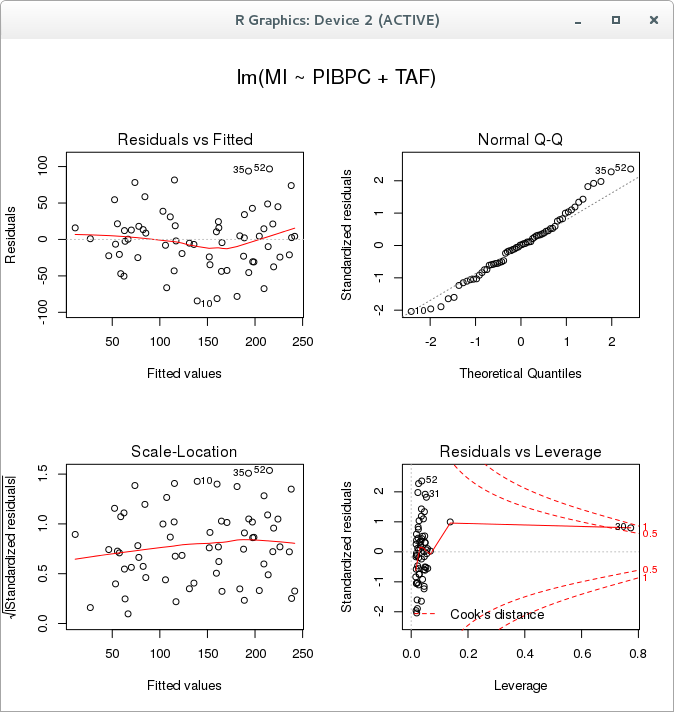
\includegraphics[width=0.9\linewidth]{analisisGraficoModelo3}\\
\caption[Titulo en el índice de figuras (opcional)]{Título en el 
documento. Las imágenes pueden ser raster (de preferencia jpg, png 
con buena resoloción para imprimir) o vectorial (convertir a pdf, en 
este caso la resolución no afecta) Fuente: imagen tomada de~\cite{liu}.}
\end{figure}


\begin{lem}\label{lmcp11}Sean $z,w \in \C$, $1 < p \leq 2$ y $1/p +
1/q = 1$. Entonces tenemos \[\abs{z+w}^q + \abs{z-w}^q \leq 2 (|z|^p
+ |w|^p)^{\frac{1}{p-1}}.\]
\end{lem}

\begin{proof} Consultar~\cite[p. 227]{Hewit}. \end{proof}

\begin{defn}\label{dfcp5}Sea $f:X\To \RR$ una aplicación. Se definen
las aplicaciones $f^+\!\df\max\{f,0\}$, $f^-\!\df-\min\{f,0\}$, a
$f^+$ y $f^-$ se les llama la \textbf{parte positiva y negativa} de
$f$, respectivamente.
\end{defn}


\begin{prp}\label{prcp2}Para cualquier aplicación $f:X\To \R$
denotaremos su valor absoluto con $\abs f$, entonces tenemos
\[\abs f=f^++f^-,\quad f=f^+-f^-.\]
\end{prp}

% --------------->  

\section{Tablas y Gráficas}

Las tablas y gráficas deben tener un título \verb|\caption{text}| que la identifique, debe especificar la \textbf{fuente}, y una etiqueta \verb|\label{text}| para hacer referencias cruzadas dentro del documento.

%% TABLAS LARGAS LLEVAN TODAS LAS DIVISIONES DE LOS BLOQUES

\begin{longtable}{|l|l|l|l|l|}
\caption[]{Diccionario de datos, tabla \textit{marn} (continuación)} \\ \hline

\multicolumn{1}{|c|}{\textbf{Name}} & \multicolumn{1}{c|}{\textbf{Data type}} & \multicolumn{1}{c|}{\textbf{Not Null?}} & \multicolumn{1}{c|}{\textbf{Primary key?}} & \multicolumn{1}{c|}{\textbf{Default}} \\ \hline \endhead
	\caption[Diccionario de datos, tabla \textit{marn}]{Diccionario de datos, tabla \textit{marn}. Fuente: obtenida de pgAdminIII}\label{data:marn} \\ \hline

	\multicolumn{1}{|c|}{\textbf{Name}} & \multicolumn{1}{c|}{\textbf{Data type}} & \multicolumn{1}{c|}{\textbf{Not Null?}} & \multicolumn{1}{c|}{\textbf{Primary key?}} & \multicolumn{1}{c|}{\textbf{Default}} \\ \hline \endfirsthead 

	id & \textit{integer} & \textit{Yes} & \textit{Yes} & \textit{nextval('marn\_id\_seq'} \\ %\hline

	 &  &  &  & \textit{::regclass)}\footnote{Note que la tabla es mas ancha que lo preestablecido. Procure diseñar elementos acordes con el espacio preestablecido.} \\ \hline

	\multicolumn{ 5}{|l|}{Clave primaria que  obtendrá su valor de forma secuencial al ingresar un nuevo registro} \\ \hline
		lista\_tax & \textit{text} & \textit{No} & \textit{No} & \textit{} \\ \hline

	\multicolumn{ 5}{|l|}{Clasificación del proyecto en base al Listado Taxativo del MARN} \\ \hline
		no\_marn & \textit{text} & \textit{No} & \textit{No} & \textit{} \\ \hline

	\multicolumn{ 5}{|l|}{Numero de expediente asignado por el MARN} \\ \hline
		date0 & \textit{date} & \textit{No} & \textit{No} & \textit{} \\ \hline

	\multicolumn{ 5}{|l|}{Día del ingreso del expediente del proyecto (instrumento ambiental) en el MARN} \\ \hline
		notas & \textit{text} & \textit{No} & \textit{No} & \textit{} \\ \hline

	\multicolumn{ 5}{|l|}{Observaciones} \\ \hline
		no\_res\_ap & \textit{text} & \textit{No} & \textit{No} & \textit{} \\ \hline

	\multicolumn{ 5}{|l|}{Numero de resolución aprobatoria del proyecto por el MARN%
	\footnote{Note que en esta línea la tabla se corta y continua en la siguiente página. 
	Utilizar paquete \textsf{longtable} y ambiente \textit{longtable}.}} \\ \hline
		date\_res\_ap & \textit{date} & \textit{No} & \textit{No} & \textit{} \\ \hline

	\multicolumn{ 5}{|l|}{Día de emisión de la resolución aprobatoria por el MARN} \\ \hline
		date0\_fianza & \textit{date} & \textit{No} & \textit{No} & \textit{} \\ \hline

	\multicolumn{ 5}{|l|}{Día de emisión de fianza del proyecto.} \\ \hline
		no\_res\_fianza & \textit{text} & \textit{No} & \textit{No} & \textit{} \\ \hline

	\multicolumn{ 5}{|l|}{Numero de la resolución de aceptación de fianza por el MARN} \\ \hline
		date1\_fianza & \textit{date} & \textit{No} & \textit{No} & \textit{} \\ \hline

	\multicolumn{ 5}{|l|}{Fecha de inicio de fianza} \\ \hline
		date2\_fianza & \textit{date} & \textit{No} & \textit{No} & \textit{} \\ \hline

	\multicolumn{ 5}{|l|}{Fecha de finalización de fianza (renovación)} \\ \hline
		lic\_ambiental & \textit{text} & \textit{No} & \textit{No} & \textit{} \\ \hline

	\multicolumn{ 5}{|l|}{Numero de licencia ambiental} \\ \hline
		date\_lic\_ambiental & \textit{date} & \textit{No} & \textit{No} & \textit{} \\ \hline

	\multicolumn{ 5}{|l|}{Fecha de finalización de ultima licencia ambiental} \\ \hline
		proyecto\_id & \textit{integer} & \textit{Yes} & \textit{No} & \textit{} \\ \hline

	\multicolumn{ 5}{|l|}{Enlace con la tabla proyecto\_id} \\ \hline
\end{longtable}


